\documentclass[cjk,xcolor=dvipsnames,fleqn]{beamer}

\graphicspath{{./figures/}}% 画像ファイルのディレクトリ
\hypersetup{unicode=true}% しおりの文字化け対策

\usepackage{luatexja,luatexja-fontspec}
\usepackage[noembed]{luatexja-preset}
\usepackage{graphicx}
\usepackage[orientation=portrait,size=a0]{beamerposter}
\usepackage{calc}%% Enable infix arithmetic operators

\usetheme{sumiilab-poster}

%% http://mix-mplus-ipa.osdn.jp/migmix/
\setsansfont[
    Path=./fonts/migmix-1p/,
    Extension=.ttf,
    Ligatures=TeX,
    BoldFont=migmix-1p-bold
]{migmix-1p-regular}
\setsansjfont[
    Path=./fonts/migmix-1p/,
    Extension=.ttf,
    Ligatures=TeX,
    BoldFont=migmix-1p-bold
]{migmix-1p-regular}

\urlstyle{sf}

%\beamertemplategridbackground[1cm]
\setbeamercolor{figure}{bg=white}

%%%
%%% LaTeX macros
%%%

\newcommand{\cdkeyword}[1]{\mathbf{#1}}%% code keyword
\newcommand{\UN}{\cdkeyword{Un}}
\newcommand{\BOOL}{\cdkeyword{Bool}}
\newcommand{\TRUE}{\cdkeyword{true}}
\newcommand{\FALSE}{\cdkeyword{false}}
\newcommand{\IF}{\cdkeyword{if}}
\newcommand{\THEN}{\cdkeyword{then}}
\newcommand{\ELSE}{\cdkeyword{else}}
\newcommand{\ABS}{\cdkeyword{abs}}
\newcommand{\APP}{\cdkeyword{app}}
\newcommand{\VAR}{\cdkeyword{var}}
\newcommand{\Item}{\structure{\textbullet}~}

\title{機械学習による関数型ブーリアンプログラムの型推論}
\author[阿部 \& 住井]{阿部晃典 \and 住井英二郎}
\institute[東北大学]{東北大学 大学院情報科学研究科}

\setbeamertemplate{headline}{%
  \leavevmode
  \begin{beamercolorbox}[wd=\textwidth]{headline}
    \vskip4ex
    \centering
    \usebeamercolor{title in headline}{%
      \usebeamerfont{title in headline}{\inserttitle}}\\[2ex]
    \raggedright\hskip.75ex
    \usebeamercolor{author in headline}{%
      \usebeamerfont{author in headline}{%
        デモ:\url{http://j.mp/MLinf}\hfill
        \insertauthor{}(東北大学)
        \hskip0ex}}
    \vskip1.5ex
  \end{beamercolorbox}
}

\begin{document}
\begin{frame}[t,fragile]{}
  \vskip-3ex
  \begin{columns}[onlytextwidth]
    \begin{column}[t]{0.5\textwidth-1ex}
      \begin{block}{はじめに}
  \structure{静的型付けの問題点}
  \hfill\Item%
  \begin{tabular}[t]{l@{}}
    型エラーの位置は論理的には\\
    曖昧で一意には特定できない
  \end{tabular}\\[0.5ex]
  \hfill\Item 高度な型は検査や推論が決定不能\\
  \structure{目標}\quad
  \begin{tabular}[t]{ll}
    \Item & 論理的手法では決定できないことを\\
          & 統計的ヒューリスティックスで解決したい\\
    \Item & 型付けに機械学習の統計的手法を導入
  \end{tabular}
\end{block}
      \vskip.5ex
      \begin{block}{準備:条件付き確率場 {\small{}[Lafferty ICML2001]}}
  \begin{itemize}
  \item 確率変数の間の複雑な依存関係をグラフで表現
  \item 自然言語処理などで用いられる確率モデル
  \end{itemize}
  \structure{具体例}:``John loves Alice'' の品詞予測
  \begin{itemize}
  \item 因子ノード(黒い四角)ごとに点数を計算
  \item \alert{合計点数が最大}となる品詞の割り当て方が正解\\(の可能性が高い)
  \end{itemize}
  \vskip-0.5\baselineskip
  \begin{columns}[onlytextwidth]
    \begin{column}[t]{0.6\textwidth}\\
      \begin{beamercolorbox}{figure}
        \centering
        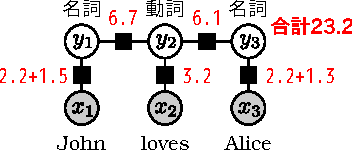
\includegraphics[height=10cm]{pos-tagging-score1.pdf}
      \end{beamercolorbox}
      \vskip\baselineskip
      \begin{beamercolorbox}{figure}
        \centering
        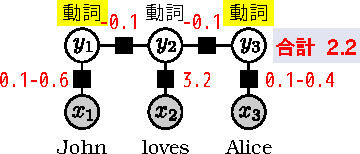
\includegraphics[height=10cm]{pos-tagging-score2.pdf}
      \end{beamercolorbox}
    \end{column}
    \begin{column}[t]{0.4\textwidth}\\
      \footnotesize
      \begin{table}
        \centering
        \begin{tabular}{l@{\hskip2em}r}
          \hline
          特徴 & 重み \\
          \hline
          $y_i = \text{名詞} \land \mathrm{CapInit}(x_i)$ & 2.2 \\
          $y_i = \text{動詞} \land \mathrm{CapInit}(x_i)$ & 0.1 \\
          $y_i = \text{名詞} \land x_i = \text{John}$ & 1.5 \\
          $y_i = \text{動詞} \land x_i = \text{John}$ & -0.6 \\
          $y_i = \text{名詞} \land x_i = \text{Alice}$ & 1.3 \\
          $y_i = \text{動詞} \land x_i = \text{Alice}$ & -0.4 \\
          $y_i = \text{名詞} \land x_i = \text{loves}$ & 0.1 \\
          $y_i = \text{動詞} \land x_i = \text{loves}$ & 3.2 \\
          \hline
          $y_i = \text{名詞} \land y_{i+1} = \text{名詞}$ & 1.3 \\
          $y_i = \text{動詞} \land y_{i+1} = \text{名詞}$ & 6.1 \\
          $y_i = \text{名詞} \land y_{i+1} = \text{動詞}$ & 6.7 \\
          $y_i = \text{動詞} \land y_{i+1} = \text{名詞}$ & -0.1 \\
          \hline
        \end{tabular}
        \caption{点数表}
      \end{table}
      \scriptsize
      ※ $\mathrm{CapInit}(x_i)$ は $x_i$ の先頭が大文字なら真
    \end{column}
  \end{columns}
\end{block}
      \vskip.5ex
      \begin{block}{特徴関数:単純型付け規則を弱めた規則}
  \vskip1ex
  \begin{tabular}{l@{~}l}
    例:
    & $\text{\textsc{T-WeakIf1}}\,
      \dfrac
      {~M : \alert{\tau'}\quad N : \tau\quad K : \tau~}
      {~\IF~M~\THEN~N~\ELSE~K : \tau~}$ \\[1em]
    & $\text{\textsc{T-WeakIf2}}\,
      \dfrac
      {~M : \BOOL\quad N : \tau\quad K : \tau~}
      {~\IF~M~\THEN~N~\ELSE~K : \alert{\tau'}~}$ \\[1em]
    & $\text{\textsc{T-WeakIf3}}\,
      \dfrac
      {~M : \BOOL\quad N : \tau\quad K : \alert{\tau'}~}
      {~\IF~M~\THEN~N~\ELSE~K : \tau~}$ \\[1em]
    & $\text{\textsc{T-WeakIf4}}\,
      \dfrac
      {~M : \BOOL\quad N : \alert{\tau'}\quad K : \tau~}
      {~\IF~M~\THEN~N~\ELSE~K : \tau~}$
  \end{tabular}
  \vskip1ex
  \begin{itemize}
  \item 型付け可能な式:\alert{弱めた規則のみ}で\alert{正しく推論}可能
    \begin{itemize}
    \item 点数最大化のため全ての規則を同時に適用し \textsc{T-If} と同じ規則になる
    \end{itemize}
  \item 型付け不可能な式:\alert{well-typed らしさ}を計算
    \begin{itemize}
    \item 型付け不可能な$\lambda$式でも可能な限り型を合わせる
    \item より多くの規則が成立すれば、点数が上がる
    \end{itemize}
  \end{itemize}
\end{block}
    \end{column}
    \begin{column}[t]{0.5\textwidth}
      \begin{block}{提案手法:条件付き確率場による単純型付け}
  (同一変数の頂点をマージした)型注釈付き AST に\\点数を付ける\\
  \structure{具体例}:$\lambda x. \IF~x~\THEN~\FALSE~\ELSE~\TRUE$
  \begin{itemize}
  \item 因子ノード(黒い四角)ごとに点数を計算
  \item \alert{合計点数が最大}となる型注釈の割り当て方が正解\\(の可能性が高い)
  \end{itemize}
  \vskip1em
  \begin{beamercolorbox}{figure}
    \raggedleft
    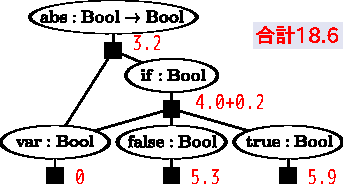
\includegraphics[height=18cm]{crf-typing-score1.pdf}
  \end{beamercolorbox}
  \vskip0.5\baselineskip
  \begin{beamercolorbox}{figure}
    \raggedleft
    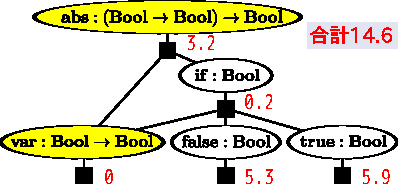
\includegraphics[height=18cm]{crf-typing-score2.pdf}
  \end{beamercolorbox}
  \vskip1em
  \begin{table}
    \centering
    \begin{tabular}{l@{\hskip1ex}r@{\hskip6ex}l@{\hskip1ex}r}\hline
      特徴{\small(型付け規則)} & 重み & 特徴{\small(型付け規則)} & 重み \\\hline
      \textsc{T-True} & 5.9 & \textsc{T-False} & 5.3 \\
      \textsc{T-Abs} & 3.2 & \textsc{T-App} & 1.7 \\
      \textsc{T-If} & 4.0 & \textsc{T-WeakIf1} & 0.2 \\\hline
    \end{tabular}
    \caption{\normalsize{}点数表}
  \end{table}
\end{block}
      \vskip.5ex
      \begin{block}{重みの学習と型推論}
  \structure{型付け規則学習}
  \begin{itemize}
  \item 入力:訓練集合(自動生成した単純型付き$\lambda$式800個)
  \item 出力:重み(型付けに有用な規則の重みは大きくなる)
  \end{itemize}
  \structure{型推論}(学習した重みを使用)
  \begin{itemize}
  \item 入力:型無し$\lambda$式
  \item 出力:点数を最大化する型注釈
    \begin{itemize}
    \item 予測可能な型注釈\\
      \begin{tabular}[t]{l}
        $\BOOL$,\quad
        $\BOOL\to\BOOL$,\\
        $\BOOL\to\BOOL\to\BOOL$, \\
        $(\BOOL\to\BOOL)\to\BOOL$
      \end{tabular}
    \end{itemize}
  \end{itemize}
\end{block}
    \end{column}
  \end{columns}
\end{frame}
\end{document}
